% Teaser: three examples (rows) x Original / SteerVTE / Banksy (columns), plus headline numbers of the 526-clip run.
\begin{strip}
\centering
\begin{minipage}[c]{0.70\linewidth}
\centering
\setlength{\tabcolsep}{1.5pt}\renewcommand{\arraystretch}{0.6}
\begin{tabular}{@{}m{1.55cm}ccc@{}}
 & \footnotesize\textbf{Original (generated)} & \footnotesize\textbf{\steer~\cite{zeng2026steervte}} & \footnotesize\textbf{\method (ours)} \\[2pt]
\scriptsize (a) garbled,\newline target \str{RECORDS} &
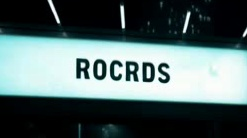
\includegraphics[width=0.28\linewidth]{figs/cells/teaser_g055_en_signboard_s6_orig.jpg} &

\includegraphics[width=0.28\linewidth]{figs/cells/teaser_g055_en_signboard_s6_steervte.jpg} &
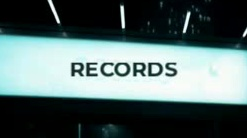
\includegraphics[width=0.28\linewidth]{figs/cells/teaser_g055_en_signboard_s6_B1.jpg} \\
 & \scriptsize\no\,\str{ROCRDS} & \scriptsize\no\,\str{RECRDS} & \scriptsize\ok\,\str{RECORDS} \\[3pt]
\scriptsize (b) garbled,\newline target \zh{便利店} &
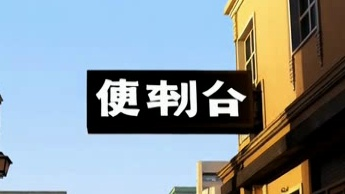
\includegraphics[width=0.28\linewidth]{figs/cells/teaser_g064_zh_screen_s7_orig.jpg} &
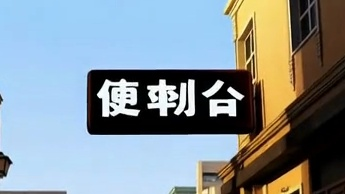
\includegraphics[width=0.28\linewidth]{figs/cells/teaser_g064_zh_screen_s7_steervte.jpg} &
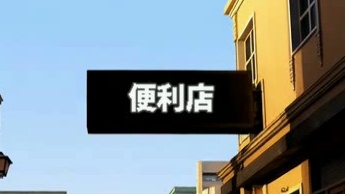
\includegraphics[width=0.28\linewidth]{figs/cells/teaser_g064_zh_screen_s7_B1.jpg} \\
 & \scriptsize\no\,\cjkimg{cjk_eab75b7f4d} & \scriptsize\no\,\cjkimg{cjk_c466d65593} & \scriptsize\ok\,\zh{便利店} \\[3pt]
\scriptsize (c) already correct,\newline target \str{FRESH BREAD} &
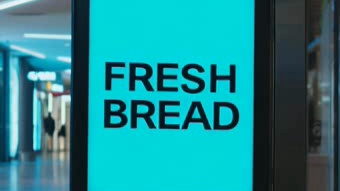
\includegraphics[width=0.28\linewidth]{figs/cells/teaser_g008_en_signboard_s2_orig.jpg} &
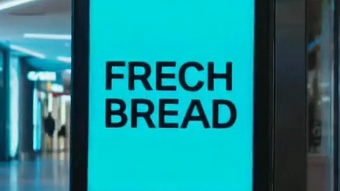
\includegraphics[width=0.28\linewidth]{figs/cells/teaser_g008_en_signboard_s2_steervte.jpg} &
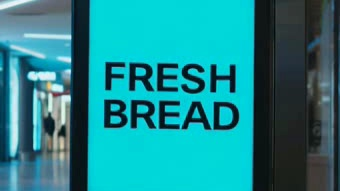
\includegraphics[width=0.28\linewidth]{figs/cells/teaser_g008_en_signboard_s2_B1.jpg} \\
 & \scriptsize\ok\,\str{FRESH BREAD} & \scriptsize\no\,\str{FRECH BREAD} & \scriptsize\ok\,\str{FRESH BREAD} (untouched) \\
\end{tabular}
\end{minipage}\hfill
\begin{minipage}[c]{0.28\linewidth}
\centering
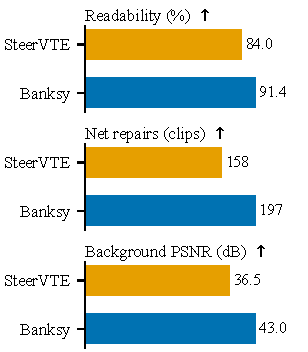
\includegraphics[width=\linewidth]{figs/plots/teaser_stats.pdf}
\end{minipage}
\captionsetup{hypcap=false}
\captionof{figure}{\textbf{Repairing garbled text in generated videos.} A generative video text editor rewrites the text region and often produces plausible but wrong characters (a, b) or breaks text that was already correct (c). \method edits only when evidence supports it, writes the target string deterministically, and leaves everything outside the text untouched. Below each crop: the transcription of frame 24 by the evaluation reader (\ok~correct, \no~wrong). Right: headline numbers on our 526-clip benchmark (\cref{sec:main}). Examples (a, b) were chosen among clips where \steer fails and \method succeeds; (c) is the only clip among the 46 that \method leaves untouched which \steer breaks.}
\captionsetup{hypcap=true}
\label{fig:teaser}
\end{strip}
